\documentclass[12pt,a4paper]{article}
\usepackage[utf8]{inputenc}
\usepackage[vietnamese]{babel}
\usepackage{amsmath,amssymb,amsfonts}
\usepackage{booktabs}
\usepackage{tabularx}
\usepackage{graphicx}
\usepackage{hyperref}
\usepackage[margin=2.5cm]{geometry}
\usepackage{enumitem}
\usepackage{float}
\usepackage{fancyvrb}
\usepackage{tcolorbox}
\usepackage{xcolor}

% Định nghĩa box cho các đoạn giải thích (blockquote)
\newtcolorbox{explain}{
  colback=blue!5!white,
  colframe=blue!40!black,
  fonttitle=\bfseries,
  left=6pt,right=6pt,top=4pt,bottom=4pt,
  boxrule=0.5pt,
  arc=2pt
}

\title{\textbf{Thuật toán Parallel BFS Hybrid} \\ \large Trình bày Lý thuyết Toán học Đầy đủ}
\author{}
\date{}

\setlength{\parindent}{0pt}
\setlength{\parskip}{6pt}

\begin{document}
\maketitle

\begin{explain}
Tài liệu này trình bày và giải thích chi tiết thuật toán BFS song song lai (Hybrid MPI + OpenMP) kết hợp kỹ thuật Direction-Optimizing từ đầu đến cuối, sử dụng ký hiệu toán học hàn lâm kết hợp diễn giải bằng lời.
\end{explain}

%======================================================================
\section{Bài toán đặt ra}
%======================================================================

\textbf{Bài toán BFS (Breadth-First Search):} Cho một đồ thị và một đỉnh nguồn, tìm \textbf{đường đi ngắn nhất} (tính theo số cạnh) từ đỉnh nguồn đến mọi đỉnh khác trong đồ thị.

\textbf{Thách thức:} Khi đồ thị có hàng triệu hoặc hàng tỷ đỉnh, một máy tính đơn lẻ không đủ sức tính toán trong thời gian hợp lý. Do đó, cần phân tán bài toán lên \textbf{nhiều máy tính} (Cluster) để nhiều máy cùng tính toán song song, nhằm giảm thời gian xử lý.

%======================================================================
\section{Thuật toán Sinh Đồ thị R-MAT}
%======================================================================

Trong dự án này, đồ thị đầu vào cho thuật toán BFS không được đọc từ file mà được \textbf{sinh tự động} bằng mô hình \textbf{R-MAT} (Recursive MATrix). Đây là mô hình tiêu chuẩn được sử dụng trong bảng xếp hạng siêu máy tính \textbf{Graph500}.

%----------------------------------------------------------------------
\subsection{Ý tưởng cốt lõi}
%----------------------------------------------------------------------

R-MAT sinh đồ thị bằng cách mô phỏng quá trình \textbf{đệ quy chia 4 góc phần tư} (recursive quadrant partitioning) trên ma trận kề $n \times n$.

Hãy tưởng tượng ta có một ma trận kề kích thước $n \times n$ (hàng đại diện cho đỉnh nguồn $u$, cột đại diện cho đỉnh đích $v$). Thay vì đặt cạnh ngẫu nhiên đều, R-MAT chia ma trận thành \textbf{4 góc phần tư} và gán xác suất khác nhau cho mỗi góc. Góc nào có xác suất cao hơn thì cạnh sẽ rơi vào đó nhiều hơn, tạo ra sự ``tập trung'' giống mạng xã hội thật.

\begin{figure}[H]
\centering
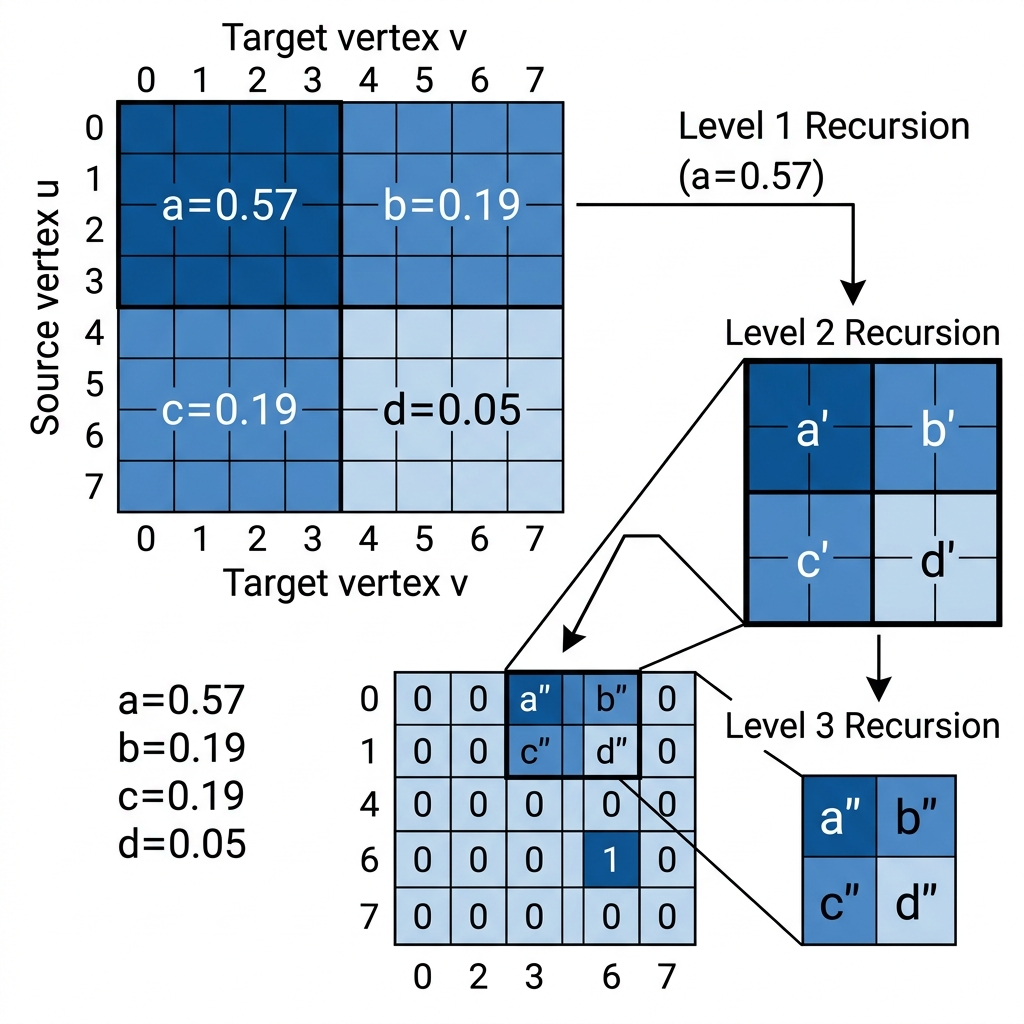
\includegraphics[width=0.85\textwidth]{rmat_illustration.png}
\caption{Minh họa thuật toán R-MAT: ma trận kề được chia đệ quy thành 4 góc với xác suất $(a, b, c, d)$. Qua mỗi vòng lặp, thuật toán chọn một góc và thu nhỏ phạm vi cho đến khi xác định được một ô duy nhất --- đó chính là cạnh $(u, v)$.}
\label{fig:rmat}
\end{figure}

%----------------------------------------------------------------------
\subsection{Tham số R-MAT}
%----------------------------------------------------------------------

Mô hình R-MAT được xác định bởi 4 tham số xác suất $(a, b, c, d)$ thỏa mãn:

\begin{equation}
a + b + c + d = 1.0, \quad a \geq b \geq c \geq d
\end{equation}

\begin{table}[H]
\centering
\begin{tabularx}{\textwidth}{clcX}
\toprule
\textbf{Tham số} & \textbf{Góc phần tư} & \textbf{Giá trị Graph500} & \textbf{Ý nghĩa} \\
\midrule
$a$ & Trên--Trái & 0.57 & Xác suất cạnh rơi vào vùng ``hub nối hub'' (đỉnh chỉ số nhỏ nối đỉnh chỉ số nhỏ). Đây là giá trị lớn nhất, tạo ra cụm đỉnh có bậc rất cao. \\
$b$ & Trên--Phải & 0.19 & Xác suất cạnh nối hub (chỉ số nhỏ) sang vùng ngoại vi (chỉ số lớn). \\
$c$ & Dưới--Trái & 0.19 & Xác suất cạnh nối ngoại vi sang hub (đối xứng với $b$). \\
$d$ & Dưới--Phải & 0.05 & Xác suất cạnh nối ngoại vi với ngoại vi. Giá trị rất nhỏ, nghĩa là vùng đỉnh chỉ số lớn rất ít kết nối với nhau. \\
\bottomrule
\end{tabularx}
\end{table}

\begin{explain}
\textbf{Tại sao $a$ lớn nhất?} Vì $a = 0.57$ (chiếm 57\% xác suất), phần lớn cạnh sẽ rơi vào góc trên--trái. Điều này có nghĩa là các đỉnh có chỉ số nhỏ (0, 1, 2, ...) sẽ được kết nối dày đặc với nhau, tạo thành các ``hub'' --- giống như những người nổi tiếng trên mạng xã hội có hàng triệu kết nối. Các đỉnh chỉ số lớn (ngoại vi) thì rất ít cạnh, giống như người bình thường chỉ có vài chục bạn bè.
\end{explain}

%----------------------------------------------------------------------
\subsection{Thuật toán Chi tiết: Sinh một Cạnh $(u, v)$}
%----------------------------------------------------------------------

\textbf{Đầu vào:} Số đỉnh $n$ (phải là lũy thừa của 2), bộ tham số $(a, b, c, d)$, bộ sinh số ngẫu nhiên.

\textbf{Đầu ra:} Một cạnh $(u, v)$ với $u, v \in \{0, 1, \ldots, n-1\}$.

\textbf{Quy trình:}

\begin{enumerate}
  \item \textbf{Khởi tạo:} Đặt $u \leftarrow 0$, $v \leftarrow 0$, $\text{step} \leftarrow n$.

  \begin{explain}
  Ban đầu, ``con trỏ'' đang ở góc trên--trái của ma trận kề, và phạm vi xét là toàn bộ ma trận $n \times n$.
  \end{explain}

  \item \textbf{Lặp} (trong khi $\text{step} > 1$):
  \begin{enumerate}[label=\alph*.]
    \item Chia đôi phạm vi: $\text{step} \leftarrow \text{step} / 2$.
    \item Sinh một số ngẫu nhiên $r \in [0, 1)$.
    \item Chọn góc phần tư dựa vào $r$:

    \begin{itemize}
      \item Nếu $r < a$: chọn góc \textbf{Trên--Trái} $\rightarrow$ $u$ và $v$ \textbf{không đổi}.

      \item Nếu $a \leq r < a + b$: chọn góc \textbf{Trên--Phải} $\rightarrow$ $v \leftarrow v + \text{step}$.

      \item Nếu $a + b \leq r < a + b + c$: chọn góc \textbf{Dưới--Trái} $\rightarrow$ $u \leftarrow u + \text{step}$.

      \item Nếu $r \geq a + b + c$: chọn góc \textbf{Dưới--Phải} $\rightarrow$ $u \leftarrow u + \text{step}$, $v \leftarrow v + \text{step}$.
    \end{itemize}
  \end{enumerate}

  \begin{explain}
  Mỗi vòng lặp thu hẹp phạm vi ma trận xuống còn $1/4$. Nếu chọn góc Trên--Trái, ta ở nguyên ô hiện tại. Nếu chọn góc khác, ta dịch chuyển ``con trỏ'' $(u, v)$ sang phần tương ứng. Sau $\log_2(n)$ vòng lặp, $\text{step} = 1$ và $(u, v)$ xác định duy nhất \textbf{một ô} trong ma trận --- đó chính là cạnh được sinh ra.
  \end{explain}

  \item \textbf{Trả về} cạnh $(u, v)$.
\end{enumerate}

%----------------------------------------------------------------------
\subsection{Ví dụ Minh họa Cụ thể}
%----------------------------------------------------------------------

Giả sử $n = 8$ (ma trận $8 \times 8$). Thuật toán chạy $\log_2(8) = 3$ vòng lặp:

\begin{table}[H]
\centering
\begin{tabularx}{\textwidth}{ccccX}
\toprule
\textbf{Vòng} & \textbf{step} & \textbf{$r$ ngẫu nhiên} & \textbf{Góc chọn} & \textbf{Kết quả} \\
\midrule
1 & $8 \rightarrow 4$ & $r = 0.35$ ($ < a = 0.57$) & Trên--Trái & $u=0, v=0$. Phạm vi thu hẹp: ô $[0{:}3] \times [0{:}3]$. \\
2 & $4 \rightarrow 2$ & $r = 0.62$ ($a \leq r < a{+}b{+}c$) & Dưới--Trái & $u = 0 + 2 = 2, v = 0$. Phạm vi: $[2{:}3] \times [0{:}1]$. \\
3 & $2 \rightarrow 1$ & $r = 0.70$ ($\geq a{+}b$) & Dưới--Trái & $u = 2 + 1 = 3, v = 0$. Ô duy nhất: $(3, 0)$. \\
\bottomrule
\end{tabularx}
\end{table}

$\Rightarrow$ Cạnh được sinh ra là $(u, v) = (3, 0)$, nghĩa là đỉnh 3 nối với đỉnh 0.

%----------------------------------------------------------------------
\subsection{Xây dựng Toàn bộ Đồ thị}
%----------------------------------------------------------------------

Để sinh đồ thị $G = (V, E)$ hoàn chỉnh, thuật toán lặp lại quá trình trên $m_{\text{target}} = n \times \text{scale\_factor}$ lần (trong đó \texttt{scale\_factor} = 16 theo cấu hình thực nghiệm). Mỗi lần sinh được một cạnh $(u, v)$.

Sau khi sinh xong, thuật toán thực hiện các bước hậu xử lý:

\begin{enumerate}
  \item \textbf{Loại bỏ self-loop:} Nếu $u = v$ thì bỏ qua cạnh đó (một đỉnh nối với chính nó là vô nghĩa trong BFS).

  \item \textbf{Thêm cạnh ngược (Undirected):} Với mỗi cạnh $(u, v)$, thêm cả cạnh $(v, u)$ vì đồ thị là vô hướng.

  \item \textbf{Sắp xếp và loại bỏ cạnh trùng lặp (Deduplication):} Sắp xếp toàn bộ danh sách cạnh theo cặp $(u, v)$ rồi loại bỏ các cạnh lặp. Đảm bảo mỗi cặp $(u, v)$ chỉ xuất hiện đúng 1 lần.

  \item \textbf{Chuyển đổi sang CSR:} Xây dựng mảng \texttt{row\_ptr} và \texttt{adj} từ danh sách cạnh đã sạch.
\end{enumerate}

%----------------------------------------------------------------------
\subsection{Tính chất của Đồ thị R-MAT}
%----------------------------------------------------------------------

Đồ thị R-MAT có các tính chất quan trọng ảnh hưởng trực tiếp đến hiệu năng song song:

\begin{itemize}
  \item \textbf{Phân bố bậc lệch (Power-law degree distribution):} Một số ít đỉnh (hub) có bậc cực lớn (hàng nghìn đến hàng triệu cạnh), trong khi đại đa số đỉnh có bậc rất thấp (chỉ vài cạnh). Tính chất này mô phỏng chính xác mạng xã hội thực.

  \item \textbf{Thế giới nhỏ (Small-world property):} Đường kính (diameter) đồ thị rất nhỏ so với $n$, thuật toán BFS chỉ cần vài level (thường 5--7 level) là duyệt hết.

  \item \textbf{Tái tạo được (Reproducible):} Nhờ sử dụng \textbf{seed} cố định ($= 42$) cho bộ sinh số ngẫu nhiên (\texttt{xorshift64}), mọi lần chạy đều sinh ra đúng cùng một đồ thị. Điều này đảm bảo tính tái lập cho thực nghiệm khoa học.

  \item \textbf{Gây khó khăn cho cân bằng tải:} Do bậc lệch, khi chia đỉnh đều cho $k$ tiến trình bằng 1D Partitioning, tiến trình quản lý vùng đỉnh chỉ số nhỏ (chứa hub) sẽ phải xử lý nhiều cạnh hơn hẳn tiến trình quản lý vùng đỉnh chỉ số lớn.
\end{itemize}


%======================================================================
\section{Các Định nghĩa và Ký hiệu Toán học}
%======================================================================
Trước khi đi vào thuật toán, ta cần thiết lập rõ ràng các khái niệm và ký hiệu sẽ sử dụng xuyên suốt tài liệu.

%----------------------------------------------------------------------
\subsection{Đồ thị}
%----------------------------------------------------------------------

\begin{table}[H]
\centering
\begin{tabularx}{\textwidth}{llX}
\toprule
\textbf{Ký hiệu} & \textbf{Ý nghĩa} & \textbf{Giải thích} \\
\midrule
$G = (V, E)$ & Đồ thị vô hướng & $V$ là tập đỉnh, $E$ là tập cạnh \\
$n = |V|$ & Số đỉnh & Tổng số đỉnh trong đồ thị \\
$m = |E|$ & Số cạnh & Tổng số cạnh (mỗi cạnh tính 2 chiều, nên thực tế lưu $2m$ entry) \\
$s \in V$ & Đỉnh nguồn & Đỉnh xuất phát của thuật toán BFS \\
\bottomrule
\end{tabularx}
\end{table}

%----------------------------------------------------------------------
\subsection{Quan hệ Lân cận}
%----------------------------------------------------------------------

\begin{equation}
N(u) = \{v \in V \mid (u, v) \in E\}
\end{equation}

Đây là \textbf{tập các đỉnh kề} (neighborhood) của đỉnh $u$, tức là tập hợp tất cả các đỉnh $v$ sao cho tồn tại cạnh nối trực tiếp giữa $u$ và $v$.

\textbf{Bậc (degree)} của đỉnh $u$ là số lượng đỉnh kề của nó:

\begin{equation}
\deg(u) = |N(u)|
\end{equation}

\begin{explain}
\textbf{Ý nghĩa thực tế:} Trong mạng xã hội, $N(u)$ là danh sách bạn bè của người $u$, và $\deg(u)$ là số bạn bè mà $u$ có.
\end{explain}

%----------------------------------------------------------------------
\subsection{Hàm Khoảng cách}
%----------------------------------------------------------------------

\begin{equation}
d: V \rightarrow \mathbb{N}_0 \cup \{-1\}
\end{equation}

Hàm $d$ gán cho mỗi đỉnh $v$ một giá trị nguyên:
\begin{itemize}
  \item $d(v) = -1$: đỉnh $v$ \textbf{chưa được thăm} (chưa tìm thấy đường đi từ $s$ đến $v$).
  \item $d(v) = k \geq 0$: đường đi ngắn nhất từ $s$ đến $v$ có độ dài đúng bằng $k$ cạnh.
\end{itemize}

\begin{explain}
\textbf{Giải thích:} Ban đầu, tất cả đỉnh đều có $d(v) = -1$ (trạng thái ``chưa biết''). Khi thuật toán khám phá được đỉnh nào, nó sẽ gán giá trị khoảng cách cụ thể cho đỉnh đó. Giá trị $-1$ được chọn vì nó luôn nhỏ hơn mọi khoảng cách hợp lệ ($\geq 0$), rất thuận tiện khi dùng phép $\max$ để gộp kết quả giữa các máy.
\end{explain}

%----------------------------------------------------------------------
\subsection{Tập Biên (Frontier)}
%----------------------------------------------------------------------

\begin{equation}
F_l \subseteq V
\end{equation}

$F_l$ là tập hợp tất cả các đỉnh nằm ở \textbf{cấp độ $l$} (level $l$) --- tức là các đỉnh có khoảng cách từ đỉnh nguồn $s$ đúng bằng $l$:

\begin{equation}
F_l = \{v \in V \mid d(v) = l\}
\end{equation}

\begin{explain}
\textbf{Hình dung:} Tưởng tượng ném một hòn đá xuống hồ nước. Gợn sóng hình tròn lan ra dần dần. $F_l$ chính là \textbf{vòng tròn gợn sóng thứ $l$} --- là ranh giới ngoài cùng của vùng đã được khám phá tại thời điểm đó. Thuật toán BFS hoạt động bằng cách liên tục đẩy vòng tròn này ra xa hơn, cho đến khi nó không thể lan rộng thêm nữa.
\end{explain}

%----------------------------------------------------------------------
\subsection{Hệ thống Phân tán}
%----------------------------------------------------------------------

\begin{table}[H]
\centering
\begin{tabularx}{\textwidth}{llX}
\toprule
\textbf{Ký hiệu} & \textbf{Ý nghĩa} & \textbf{Giải thích} \\
\midrule
$k$ & Số tiến trình MPI & Tổng số tiến trình chạy trên Cluster \\
$P = \{p_0, p_1, \ldots, p_{k-1}\}$ & Tập các tiến trình & Mỗi $p_i$ là một tiến trình MPI chạy trên một trong 3 máy \\
$V_i$ & Phần đỉnh của $p_i$ & Tập hợp con các đỉnh mà tiến trình $p_i$ chịu trách nhiệm tính toán \\
\bottomrule
\end{tabularx}
\end{table}

%----------------------------------------------------------------------
\subsection{Biểu diễn Dữ liệu: CSR (Compressed Sparse Row)}
%----------------------------------------------------------------------

Đồ thị $G$ được lưu trữ trong bộ nhớ bằng cấu trúc \textbf{CSR} gồm 2 mảng:

\begin{itemize}
  \item \texttt{row\_ptr} (kích thước $n + 1$): Mảng con trỏ hàng. Các đỉnh kề của đỉnh $u$ được lưu liên tiếp trong mảng \texttt{adj} tại các vị trí từ \texttt{row\_ptr[u]} đến \texttt{row\_ptr[u+1] - 1}.
  \item \texttt{adj} (kích thước $m$): Mảng danh sách kề. Chứa tất cả các đỉnh kề, nối tiếp nhau.
\end{itemize}

Hay biểu diễn bằng toán học:
\begin{equation}
N(u) = \{\texttt{adj}[j] \mid j \in [\texttt{row\_ptr}[u],\; \texttt{row\_ptr}[u+1])\}
\end{equation}

\begin{explain}
\textbf{Tại sao dùng CSR?} Đồ thị R-MAT rất thưa (sparse) --- số cạnh $m \ll n^2$. Ma trận kề sẽ tốn $O(n^2)$ bộ nhớ với phần lớn là số 0. CSR chỉ tốn $O(n + m)$ và cho phép truy xuất danh sách lân cận trong $O(1)$ bước, tối ưu hóa hiệu suất cache.
\end{explain}

%----------------------------------------------------------------------
\subsection{Biểu diễn Tập Biên: Bitmap}
%----------------------------------------------------------------------

Tập $F_l$ được biểu diễn bằng một \textbf{mảng bitmap} $B$ có $\lceil n / 64 \rceil$ từ máy (word) 64-bit:

\begin{equation}
v \in F_l \iff B\left[\lfloor v / 64 \rfloor\right] \;\&\; (1 \ll (v \bmod 64)) \neq 0
\end{equation}

\begin{explain}
\textbf{Giải thích đơn giản:} Mỗi đỉnh $v$ được gán 1 bit trong mảng. Bit $= 1$ nghĩa là đỉnh đó đang nằm trong Frontier, bit $= 0$ nghĩa là không. Lý do dùng bitmap: (1) tra cứu $O(1)$, (2) hợp nhất giữa các máy cực kỳ nhanh bằng phép OR bitwise.
\end{explain}

%======================================================================
\section{Phân rã Dữ liệu (Data Decomposition)}
%======================================================================

%----------------------------------------------------------------------
\subsection{Sao chép Đồ thị (Graph Replication)}
%----------------------------------------------------------------------

Toàn bộ cấu trúc CSR của đồ thị $G$ (gồm \texttt{row\_ptr} và \texttt{adj}) được \textbf{sao chép y hệt} vào bộ nhớ RAM của \textbf{tất cả} $k$ tiến trình trên cả 3 máy.

\begin{explain}
\textbf{Tại sao?} Trong quá trình tính toán, tiến trình $p_i$ cần truy xuất danh sách lân cận $N(v)$ của các đỉnh $v$ bất kỳ (kể cả những đỉnh không thuộc $V_i$). Nếu đồ thị bị chia nhỏ, tiến trình sẽ phải gửi yêu cầu \texttt{MPI\_Send/Recv} sang máy khác để hỏi ``đỉnh $v$ có những đỉnh kề nào?'' --- rất chậm. Nhờ sao chép, mọi tiến trình đều có bản đồ thị đầy đủ trong RAM cục bộ, tra cứu tức thì mà không cần giao tiếp mạng.
\end{explain}

%----------------------------------------------------------------------
\subsection{Phân hoạch Tập đỉnh (1D Block Partitioning)}
%----------------------------------------------------------------------

Tập đỉnh $V = \{0, 1, \ldots, n-1\}$ được \textbf{phân hoạch} thành $k$ phần \textbf{rời nhau} (không giao nhau), mỗi phần giao cho một tiến trình:

\begin{equation}
V_i = \left[\left\lfloor \frac{n \cdot i}{k} \right\rfloor, \;\; \left\lfloor \frac{n \cdot (i+1)}{k} \right\rfloor \right)
\end{equation}

Tính chất phân hoạch đảm bảo:
\begin{itemize}
  \item \textbf{Bao phủ toàn bộ:} $\displaystyle\bigcup_{i=0}^{k-1} V_i = V$ (mọi đỉnh đều có người chịu trách nhiệm).
  \item \textbf{Không trùng lặp:} $V_i \cap V_j = \emptyset, \;\forall i \neq j$ (không có đỉnh nào bị hai tiến trình cùng tính).
\end{itemize}

\begin{explain}
\textbf{Giải thích:} Giả sử $n = 800{,}000$ đỉnh, $k = 8$ tiến trình. Thì: $p_0$ quản lý đỉnh $[0, 100{,}000)$; $p_1$ quản lý $[100{,}000, 200{,}000)$, v.v. Mỗi tiến trình chỉ \textbf{tính toán và cập nhật} giá trị $d(v)$ cho các đỉnh $v \in V_i$ thuộc phần của mình (Owner-Computes Rule).
\end{explain}

%======================================================================
\section{Thuật toán Chi tiết Từng Bước}
%======================================================================

%----------------------------------------------------------------------
\subsection{Bước 1: Khởi tạo (Initialization)}
%----------------------------------------------------------------------

Mỗi tiến trình $p_i \in P$ thực hiện \textbf{đồng thời} và \textbf{độc lập} các bước sau:

\begin{enumerate}
  \item \textbf{Khởi tạo khoảng cách:}
  \begin{equation}
  d(v) \leftarrow -1, \quad \forall v \in V
  \end{equation}
  \begin{explain}
  Đánh dấu tất cả đỉnh là ``chưa thăm''.
  \end{explain}

  \item \textbf{Gán đỉnh nguồn:}
  \begin{equation}
  d(s) \leftarrow 0
  \end{equation}
  \begin{explain}
  Đỉnh nguồn $s$ có khoảng cách đến chính nó bằng 0.
  \end{explain}

  \item \textbf{Khởi tạo Frontier:}
  \begin{equation}
  F_0 \leftarrow \{s\}
  \end{equation}
  \begin{explain}
  Ban đầu, vòng sóng chỉ chứa mỗi mình đỉnh nguồn.
  \end{explain}

  \item \textbf{Khởi tạo biến đếm:}
  \begin{equation}
  l \leftarrow 1, \quad m_{unvisited} \leftarrow m
  \end{equation}
  \begin{explain}
  $l$ là cấp độ hiện tại (sẽ gán cho các đỉnh mới khám phá). $m_{unvisited}$ là tổng số cạnh chưa bị duyệt qua, ban đầu bằng toàn bộ số cạnh.
  \end{explain}
\end{enumerate}

%----------------------------------------------------------------------
\subsection{Bước 2: Vòng lặp Duyệt theo Cấp độ (Level-synchronous Loop)}
%----------------------------------------------------------------------

Vòng lặp chính của thuật toán. Tại mỗi cấp độ $l$, thuật toán đẩy ``vòng sóng'' $F_l$ ra xa thêm một bước, sinh ra vòng sóng mới $F_{l+1}$.

\textbf{Điều kiện dừng:} Vòng lặp tiếp tục chừng nào $F_l \neq \emptyset$ (còn đỉnh để khám phá).

%......................................................................
\subsubsection{Bước 2.1: Đánh giá Heuristic --- Quyết định Hướng duyệt (Direction-Optimizing)}
%......................................................................

Đây là bước \textbf{thông minh nhất} của thuật toán, dựa trên nghiên cứu của Beamer et al. (2012). Mục đích: chọn chiến lược duyệt tối ưu nhất cho cấp độ hiện tại.

\textbf{Ý tưởng cốt lõi:} Không phải lúc nào cũng nên duyệt theo cùng một cách. Tùy theo kích thước Frontier, có lúc duyệt xuôi (Top-Down) hiệu quả hơn, có lúc duyệt ngược (Bottom-Up) hiệu quả hơn.

\textbf{Thực hiện tính toán:}

Mỗi tiến trình $p_i$ đếm \textbf{cục bộ} tổng số cạnh đang nối ra từ các đỉnh Frontier mà nó có trong phần dữ liệu:

\begin{equation}
c_i = \sum_{u \in F_l} \deg(u)
\end{equation}

\begin{explain}
Mỗi tiến trình tính tổng bậc của tất cả đỉnh đang nằm trong Frontier. Đây là số cạnh mà thuật toán sẽ phải kiểm tra nếu duyệt theo kiểu Top-Down.
\end{explain}

Sau đó, gộp tổng từ tất cả các tiến trình bằng phép \textbf{Reduction toàn cục} (Global Sum):

\begin{equation}
C = \sum_{i=0}^{k-1} c_i \quad \text{(thông qua \texttt{MPI\_Allreduce} với \texttt{MPI\_SUM})}
\end{equation}

\begin{explain}
Hàm \texttt{MPI\_Allreduce(MPI\_SUM)} sẽ cộng các giá trị $c_i$ của tất cả tiến trình lại, và kết quả $C$ được phân phối ngược lại cho mọi tiến trình.
\end{explain}

\textbf{Quy tắc quyết định:}

Thuật toán duy trì một biến trạng thái xác định đang duyệt theo hướng nào. Hai hằng số $\alpha = 14$ và $\beta = 24$ được chọn theo nghiên cứu gốc:

\begin{itemize}
  \item \textbf{Nếu đang ở chế độ Top-Down}, kiểm tra:
  \begin{equation}
  C > \frac{m_{unvisited}}{\alpha}
  \end{equation}
  \begin{itemize}
    \item Nếu \textbf{đúng} $\rightarrow$ \textit{Frontier đang bùng nổ quá lớn, sẽ phải kiểm tra rất nhiều cạnh một cách lãng phí} $\rightarrow$ Chuyển sang \textbf{Bottom-Up}.
    \item Nếu \textbf{sai} $\rightarrow$ Giữ nguyên \textbf{Top-Down}.
  \end{itemize}

  \item \textbf{Nếu đang ở chế độ Bottom-Up}, kiểm tra:
  \begin{equation}
  |F_l| \geq \frac{n}{\beta}
  \end{equation}
  \begin{itemize}
    \item Nếu \textbf{đúng} $\rightarrow$ \textit{Frontier vẫn còn lớn} $\rightarrow$ Giữ nguyên \textbf{Bottom-Up}.
    \item Nếu \textbf{sai} $\rightarrow$ \textit{Frontier đã thu nhỏ đủ rồi} $\rightarrow$ Quay lại \textbf{Top-Down}.
  \end{itemize}
\end{itemize}

\begin{explain}
\textbf{Giải thích trực giác:} Hãy tưởng tượng bạn đang tìm kiếm một người trong thành phố. Nếu bạn chỉ biết vài người (Frontier nhỏ), bạn sẽ hỏi từng người đó ``bạn quen ai?'' (Top-Down). Nhưng nếu bạn đã biết hầu hết cư dân (Frontier khổng lồ), thì thay vì hỏi hàng triệu người đã biết, tốt hơn là đi đến từng người lạ còn lại và hỏi ``bạn có quen ai trong danh sách không?'' (Bottom-Up) --- vì số người lạ bây giờ rất ít.
\end{explain}

%......................................................................
\subsubsection{Bước 2.2: Tính toán Cục bộ Song song (Local Parallel Computation)}
%......................................................................

Đây là pha mà mỗi tiến trình \textbf{tính toán độc lập} (không giao tiếp mạng). Mục tiêu: sinh ra tập biên tiếp theo $F_{l+1}$.

Khởi tạo: $F_{l+1}^{(i)} \leftarrow \emptyset$ (tập biên mới của tiến trình $i$, ban đầu rỗng).

\paragraph{Trường hợp A: Top-Down (Duyệt xuôi)}

\textbf{Ý tưởng:} ``Đi từ Frontier ra ngoài'' --- Lấy từng đỉnh đã biết trong Frontier, xem nó có hàng xóm nào chưa được thăm không.

\textbf{Mô tả toán học:} Chia tập $F_l$ thành các phần bằng nhau cho $k$ tiến trình. Tiến trình $p_i$ xử lý phần frontier từ vị trí $\lfloor |F_l| \cdot i / k \rfloor$ đến $\lfloor |F_l| \cdot (i+1) / k \rfloor$.

Bên trong tiến trình $p_i$, các luồng OpenMP \textbf{chia nhau} duyệt song song các đỉnh frontier được giao:

\begin{align}
&\forall u \in \text{(phần frontier của } p_i\text{)}: \notag \\
&\quad \forall v \in N(u): \notag \\
&\quad\quad \text{Nếu } d(v) = -1: \notag \\
&\quad\quad\quad d(v) \leftarrow l \notag \\
&\quad\quad\quad F_{l+1}^{(i)} \leftarrow F_{l+1}^{(i)} \cup \{v\}
\end{align}

\begin{explain}
\textbf{Diễn giải bằng lời:} Với mỗi đỉnh $u$ trong Frontier (những đỉnh vừa được tìm thấy ở bước trước), thuật toán lần lượt nhìn vào từng đỉnh kề $v$ của $u$. Nếu $v$ chưa từng được thăm (giá trị $d(v)$ vẫn bằng $-1$), thì:
\begin{itemize}
  \item Gán khoảng cách cho $v$: $d(v) = l$ (đỉnh $v$ cách đỉnh nguồn đúng $l$ bước).
  \item Đưa $v$ vào tập Frontier mới để xử lý tiếp ở bước sau.
\end{itemize}
\end{explain}

\begin{explain}
\textbf{Xử lý xung đột giữa các luồng (Race Condition):} Nhiều luồng OpenMP có thể đồng thời phát hiện cùng một đỉnh $v$ chưa thăm (từ các đỉnh $u$ khác nhau). Để tránh ghi đè lẫn nhau, code sử dụng \textbf{Compare-And-Swap (CAS) nguyên tử}: \texttt{\_\_sync\_val\_compare\_and\_swap(\&dist[v], -1, level)}. Phép toán này đảm bảo chỉ DUY NHẤT MỘT luồng thành công ghi $d(v)$, các luồng còn lại sẽ phát hiện $d(v)$ đã bị thay đổi và bỏ qua.
\end{explain}

\paragraph{Trường hợp B: Bottom-Up (Duyệt ngược)}

\textbf{Ý tưởng:} ``Đi từ ngoài vào Frontier'' --- Thay vì duyệt từ Frontier ra, đi ngược lại: quét tất cả các đỉnh chưa thăm, xem nó có hàng xóm nào đang nằm trong Frontier không.

\textbf{Mô tả toán học:} Tiến trình $p_i$ quét \textbf{toàn bộ dải đỉnh} mà nó sở hữu $V_i = [\text{local\_start}, \text{local\_end})$:

\begin{align}
&\forall u \in V_i \text{ thỏa mãn } d(u) = -1: \notag \\
&\quad \text{Nếu } \exists v \in N(u) \text{ sao cho } v \in F_l: \notag \\
&\quad\quad d(u) \leftarrow l \notag \\
&\quad\quad F_{l+1}^{(i)} \leftarrow F_{l+1}^{(i)} \cup \{u\} \notag \\
&\quad\quad \textbf{break} \text{ (dừng xét các } v \text{ còn lại --- Symmetry Breaking)}
\end{align}

\begin{explain}
\textbf{Diễn giải bằng lời:} Thuật toán quét từng đỉnh $u$ chưa thăm trong phần dữ liệu của mình. Với mỗi đỉnh $u$ như vậy, nó nhìn ngược vào danh sách hàng xóm $N(u)$ để tìm xem có ai trong đó đang nằm sẵn trong Frontier không. Nếu tìm thấy \textbf{dù chỉ một} hàng xóm $v$ nằm trong Frontier, lập tức:
\begin{itemize}
  \item Gán $d(u) = l$.
  \item Đưa $u$ vào Frontier mới.
  \item \textbf{Dừng ngay (break)}, không cần kiểm tra thêm các hàng xóm còn lại.
\end{itemize}
\end{explain}

\begin{explain}
\textbf{Tại sao ``break'' lại quan trọng (Symmetry Breaking)?} Vì ta chỉ cần biết ``đỉnh $u$ có đường đến Frontier không?'' --- câu trả lời là Có hoặc Không. Ngay khi tìm thấy câu trả lời Có (một hàng xóm trong Frontier), việc kiểm tra thêm là hoàn toàn dư thừa. Kỹ thuật này \textbf{cực kỳ hiệu quả} vì khi Frontier rất lớn (chiếm phần lớn đồ thị), xác suất tìm thấy một hàng xóm trong Frontier ngay ở vài bước đầu tiên là rất cao, tiết kiệm hàng triệu phép so sánh thừa.
\end{explain}

\begin{explain}
\textbf{Tại sao Bottom-Up hiệu quả khi Frontier lớn?} Khi Frontier chứa hàng triệu đỉnh, phương pháp Top-Down phải duyệt hàng triệu đỉnh $\times$ hàng nghìn hàng xóm $=$ hàng tỷ cạnh. Trong khi đó, Bottom-Up chỉ quét các đỉnh \textbf{chưa thăm} (số lượng ít khi Frontier lớn) và dừng ngay khi tìm thấy 1 liên kết. Tổng số phép tính giảm đi hàng chục lần.
\end{explain}

%......................................................................
\subsubsection{Bước 2.3: Đồng bộ hóa Toàn cục (Global Synchronization)}
%......................................................................

Sau pha tính toán cục bộ, mỗi tiến trình $p_i$ chỉ có:
\begin{itemize}
  \item Mảng $d^{(i)}(v)$ với \textbf{một phần} đã được cập nhật (phần đỉnh của $p_i$), phần còn lại vẫn giữ giá trị cũ $-1$.
  \item Tập biên cục bộ $F_{l+1}^{(i)}$ chỉ chứa các đỉnh do $p_i$ phát hiện.
\end{itemize}

Bây giờ cần \textbf{hợp nhất} kết quả từ tất cả $k$ tiến trình lại.

\textbf{Phép đồng bộ 1: Hợp nhất Mảng khoảng cách}

\begin{equation}
d(v) \leftarrow \max_{j=0}^{k-1} d^{(j)}(v), \quad \forall v \in V
\end{equation}

\begin{explain}
Thực hiện qua \texttt{MPI\_Allreduce(MPI\_IN\_PLACE, dist, n, MPI\_INT, MPI\_MAX, MPI\_COMM\_WORLD)}.

\textbf{Giải thích tại sao dùng MAX:} Với mỗi đỉnh $v$, chỉ có duy nhất 1 tiến trình (tiến trình sở hữu $v$) đã gán $d(v) = l > 0$. Tất cả các tiến trình khác vẫn giữ $d(v) = -1$. Phép $\max(-1, -1, \ldots, l, \ldots, -1) = l$. Vậy kết quả đúng sẽ được truyền đến tất cả các máy.

\textbf{Hậu quả quan trọng:} Sau bước này, \textbf{mọi} tiến trình trên cả 3 máy đều có \textbf{cùng một mảng $d(v)$ hoàn chỉnh và giống hệt nhau}. Đây là bất biến (invariant) cốt lõi của thuật toán.
\end{explain}

\textbf{Phép đồng bộ 2: Hợp nhất Tập biên}

\begin{equation}
F_{l+1} \leftarrow \bigcup_{i=0}^{k-1} F_{l+1}^{(i)}
\end{equation}

\begin{explain}
Thực hiện qua \texttt{MPI\_Allreduce(MPI\_IN\_PLACE, bitmap, nwords, MPI\_UINT64\_T, MPI\_BOR, MPI\_COMM\_WORLD)}.

\textbf{Giải thích:} Mỗi tiến trình có một mảng bitmap riêng, trong đó bit $v = 1$ nếu $p_i$ tìm thấy đỉnh $v$ ở bước vừa rồi. Phép \textbf{OR} bitwise trên tất cả các bitmap sẽ gộp tất cả các đỉnh mới tìm được lại thành một Frontier duy nhất. Nếu $p_2$ tìm thấy đỉnh 5 và $p_7$ tìm thấy đỉnh 42, thì sau OR, cả bit 5 lẫn bit 42 đều bằng 1 ở mọi tiến trình.
\end{explain}

\textbf{Tính chất Rào cản (Barrier):} Cả hai lệnh \texttt{MPI\_Allreduce} đều là \textbf{Blocking} (chặn): tiến trình nào tính xong trước bắt buộc phải \textbf{đứng chờ} cho đến khi tiến trình chậm nhất hoàn thành. Sau đó, tất cả mới đồng loạt nhận kết quả đã hợp nhất và tiến sang bước tiếp theo. Đây chính là cơ chế \textbf{Global Barrier} đảm bảo tính đồng bộ tuyệt đối.

\begin{explain}
\textbf{Chi phí:} Mỗi lần gọi, hệ thống phải truyền mảng kích thước $O(n)$ qua mạng LAN giữa 3 máy. Đây là nguyên nhân chính gây thắt cổ chai hiệu năng (bottleneck), vì tốc độ mạng LAN chậm hơn nhiều lần so với tốc độ CPU.
\end{explain}

%......................................................................
\subsubsection{Bước 2.4: Cập nhật và Chuyển cấp độ}
%......................................................................

\begin{equation}
m_{unvisited} \leftarrow m_{unvisited} - \sum_{u \in F_{l+1}} \deg(u)
\end{equation}

\begin{explain}
Trừ đi số cạnh gắn với các đỉnh vừa mới được thăm, cập nhật lại lượng cạnh chưa xử lý.
\end{explain}

\begin{equation}
F_l \leftarrow F_{l+1}
\end{equation}

\begin{explain}
``Vòng sóng mới'' trở thành ``vòng sóng hiện tại'' cho bước tiếp theo.
\end{explain}

\begin{equation}
l \leftarrow l + 1
\end{equation}

\begin{explain}
Tăng cấp độ lên 1.
\end{explain}

Sau đó, quay lại \textbf{Bước 2.1} để bắt đầu cấp độ mới.

%----------------------------------------------------------------------
\subsection{Bước 3: Kết thúc (Termination)}
%----------------------------------------------------------------------

Thuật toán dừng tại cấp độ $l_{max}$ khi:

\begin{equation}
F_{l_{max}} = \emptyset
\end{equation}

\begin{explain}
Tức là: vòng sóng ngoài cùng không chứa đỉnh nào nữa --- mọi đỉnh có thể đến được từ $s$ đều đã được thăm hết.
\end{explain}

\textbf{Đầu ra:} Mảng $d(v)$ hoàn chỉnh trên tất cả tiến trình, chứa khoảng cách đường đi ngắn nhất từ $s$ đến mọi $v \in V$:
\begin{itemize}
  \item $d(v) \geq 0$ : Đỉnh $v$ đến được từ $s$, khoảng cách đúng bằng $d(v)$.
  \item $d(v) = -1$ : Đỉnh $v$ không thể đến được từ $s$ (nằm ở thành phần liên thông khác).
\end{itemize}

Tiến trình $p_0$ (Rank 0) chịu trách nhiệm xuất kết quả cuối cùng (in ra màn hình hoặc lưu file CSV).

%======================================================================
\section{Tổng hợp: Dòng chảy Toàn bộ Thuật toán}
%======================================================================

\begin{Verbatim}[fontsize=\small]
+-----------------------------------------------------------+
|  KHỞI TẠO: d(v)<--1  ∀v;  d(s)<-0;  F₀<-{s};  l<-1      |
+----------------------------+------------------------------+
                             |
                             v
                     +---------------+     Có
                     |  F_l ≠ ∅ ?    |---------------------------+
                     +-------+-------+                           |
                             | Không                             v
                             v                   +---------------------------+
                     +---------------+           | 2.1. Đếm cạnh biên       |
                     |   KẾT THÚC   |           |      c_i = Σ deg(u)       |
                     |  Xuất d(v)    |           | C = Allreduce(SUM)        |
                     +---------------+           +-----------+---------------+
                                                             v
                                                 +---------------------------+
                                                 | C > m_unvisited / α ?     |
                                                 +-----+---------------+-----+
                                                  Có   |               | Không
                                                       v               v
                                                +----------+     +----------+
                                                |BOTTOM-UP |     | TOP-DOWN |
                                                |quét V_i  |     |quét F_l  |
                                                |d(u)=-1?  |     |xét N(u)  |
                                                |∃v∈N(u)   |     |d(v)=-1?  |
                                                | trong F? |     |gán d(v)=l|
                                                |-> break  |     |          |
                                                +----+-----+     +----+-----+
                                                     |                 |
                                                     v                 v
                                              +------------------------------+
                                              | 2.3. ĐỒNG BỘ TOÀN CỤC      |
                                              | d(v) <- Allreduce(MAX)       |
                                              | F_{l+1} <- Allreduce(BOR)    |
                                              +-------------+----------------+
                                                            v
                                              +------------------------------+
                                              | 2.4. F_l <- F_{l+1}; l<-l+1 |
                                              +-------------+----------------+
                                                            |
                                              Quay lại kiểm tra F_l ≠ ∅ ?
\end{Verbatim}

%======================================================================
\section{Phân tích Độ phức tạp}
%======================================================================

\begin{table}[H]
\centering
\begin{tabularx}{\textwidth}{lX}
\toprule
\textbf{Thành phần} & \textbf{Độ phức tạp trên mỗi Level} \\
\midrule
Tính toán Top-Down (tiến trình $p_i$) & $O\left(\dfrac{|F_l|}{k} \cdot \overline{\deg}\right)$ --- chia đều Frontier cho $k$ tiến trình \\[8pt]
Tính toán Bottom-Up (tiến trình $p_i$) & $O\left(\dfrac{n}{k}\right)$ --- quét toàn bộ dải đỉnh, nhưng break sớm \\[8pt]
Giao tiếp mạng (Allreduce) & $O(n \cdot \log k)$ --- broadcast mảng kích thước $n$ qua $k$ máy \\
\bottomrule
\end{tabularx}
\end{table}

\begin{explain}
\textbf{Nhận xét quan trọng:} Chi phí giao tiếp $O(n \log k)$ \textbf{không phụ thuộc} vào việc đang duyệt Top-Down hay Bottom-Up. Nó xảy ra ở cuối \textbf{mỗi} level. Với đồ thị lớn ($n$ lớn) trên mạng LAN chậm, chi phí này lấn át hoàn toàn thời gian tính toán --- đây chính là nguyên nhân cốt lõi khiến Speedup tổng thể $S(P)$ sụp đổ trong thực nghiệm.
\end{explain}

%======================================================================
\section{Tổng hợp Các Kỹ thuật Song song}
%======================================================================

\begin{table}[H]
\centering
\begin{tabularx}{\textwidth}{clX>{\raggedright\arraybackslash}X}
\toprule
\textbf{\#} & \textbf{Kỹ thuật} & \textbf{Tầng áp dụng} & \textbf{Mục đích} \\
\midrule
1 & MPI (Distributed Memory) & Giữa 3 máy & Giao tiếp và đồng bộ dữ liệu qua mạng LAN \\
2 & OpenMP (Shared Memory) & Bên trong mỗi máy & Tận dụng đa nhân CPU (4 hoặc 2 cores) \\
3 & 1D Block Partitioning & Chia tập đỉnh & Phân công đều đỉnh cho tiến trình \\
4 & Graph Replication & Dữ liệu đồ thị & Loại bỏ giao tiếp Point-to-Point \\
5 & Direction-Optimizing & Quyết định hướng & Cắt giảm số cạnh phải kiểm tra \\
6 & Bitmap Frontier & Biểu diễn tập biên & Tra cứu $O(1)$, merge bằng OR \\
7 & CAS Atomic & Tránh Race Condition & Đảm bảo chỉ 1 thread ghi vào $d(v)$ \\
8 & Dynamic Scheduling & Cân bằng tải OpenMP & Luồng xong sớm tự bốc việc tiếp \\
9 & MPI\_Allreduce (MAX, BOR, SUM) & Đồng bộ toàn cục & Hợp nhất kết quả từ 3 máy \\
\bottomrule
\end{tabularx}
\end{table}

\end{document}
